\documentclass{beamer}

\newcommand{\week}{Intro}

\title{Introduction to the Financial System}
\author{Econ 457}
\date{\week}

% Reference the shared preamble
\input{preamble}

% Set the footer -- change 
\setbeamertemplate{footline}{
  \leavevmode%
  \vspace{2ex}
  \hbox{%
    % Left box: Econ 457
    \begin{beamercolorbox}[wd=.4\paperwidth,ht=2.5ex,dp=1ex,left]{author in head/foot}%
      \hspace{1em}Econ 457
    \end{beamercolorbox}%
    % Middle box: Week
    \begin{beamercolorbox}[wd=.2\paperwidth,ht=2.5ex,dp=1ex,center]{date in head/foot}%
      \centering\week
    \end{beamercolorbox}%
    % Right box: Slide numbers
    \begin{beamercolorbox}[wd=.4\paperwidth,ht=2.5ex,dp=1ex,center]{date in head/foot}%
      \hfill\insertframenumber{} 
    \end{beamercolorbox}%
  }%
  \vskip0pt%
}

\begin{document}

\frame{\titlepage}

% 1
\begin{frame}
    \frametitle{Outline}
    \begin{enumerate}
        \item Introductions
        \item Economics 457
        \item Some interesting charts
    \end{enumerate}
\end{frame}

% 2
\begin{frame}[t]
    \section{Introductions}
    \frametitle{1. Introductions}
    John Bellows (me)
    \begin{itemize}
        \item Western Asset Management, 2012-2024
        \begin{itemize}
            \item Portfolio Manager, Fixed Income Portfolios
            \item Investment Strategy Committees, Responsible for Fed View
        \end{itemize}
        \item US Department of Treasury, 2009-2011
        \item PhD in Economics, UC Berkeley, 2009
    \end{itemize}
    \vspace{2em}
    Quiz (not graded, do your best!)
\end{frame}

\begin{frame}[t]
    \frametitle{1. Introductions}

    \centering
    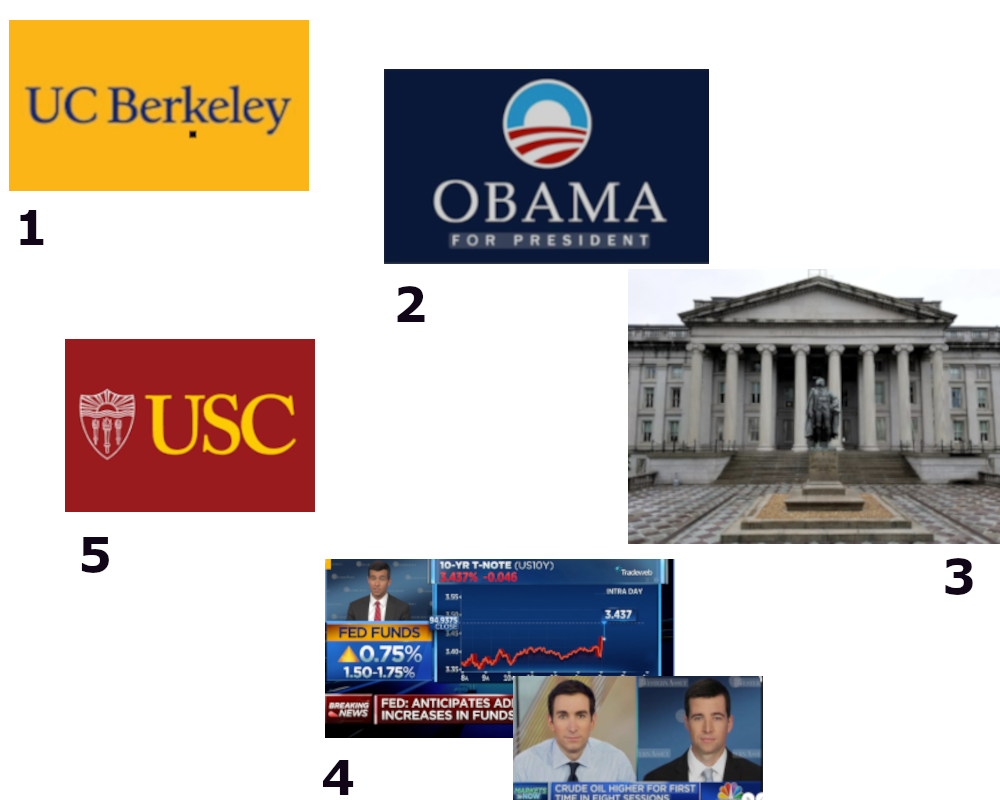
\includegraphics[width=0.8\textwidth]{figures/JB Photos.png}

\end{frame}

\begin{frame}[t]
    \frametitle{1. Introductions}

    \textbf{Office Hours:} \\
    Location: KAP 304\\
    Time: Thursdays, 1:00 - 2:00 pm\\
    Please email me if you need to meet at a different time.  I'll do my best to accommodate.\\
    \vspace{1em}
    \textbf{Email policy:} Best to talk to me during office hours or after class, especially for questions about class material or test preparation.   I will do my best to respond to emails within 24 hours.   

\end{frame}

\begin{frame}[t]
    \frametitle{1. Introductions}

    Answers to the Quiz
    \begin{enumerate}
        \item Secretary of the Treasury:
        \item Federal Reserve Chair:
        \item Current Level of Fed Funds Rate: 
        \item Range of 10-year US Treasury yields since 2020: 
        \item S\&P Year-to-date:
        \item Annualized S\&P gain since 2020: 
    \end{enumerate}

\end{frame}

\begin{frame}[t]
    \frametitle{2. Economics 457}
    \section{Economics 457}
    \framesubtitle{Material Covered}

    Goals for the class:
    \begin{itemize}
        \item Develop some basic tools used in finance
        \item Apply these tools
        \item Appreciate some of the cool results in finance
        \item Understand why finance matters
    \end{itemize}
    \vspace{1em}

    My own experience includes academia, public policy, and investing.   The material in this class will touch on all of these at different points.

\end{frame}

\begin{frame}[t]
    \frametitle{2. Economics 457}
    \framesubtitle{Material Covered}

    \vspace{-1em}

        \begin{table}
        \centering
        \footnotesize  % Global font size for the table
        \begin{tblr}{
            colspec = {Q[l,wd=2cm] Q[c,wd=2cm] Q[l,wd=6cm]}
        }
        \toprule
        Subject & Weeks & Sub-topics \\
        \midrule
        Intro & 1 \& 2 & Returns: Measurement, Distributions and Evaluation \\
        Portfolio Construction & 3, 4 & Capital Allocation, Diversification \\
        Market Equilibrium & 5-8 & CAPM, Fama-French Factors, Efficient Markets \\
        Fixed Income & 9 \& 10 & Prices, Yields, Yield Curve, Duration and Convexity \\
        Equity & 11 \& 12 & Dividend Discount Models, Price-Earnings Ratios\\
        Derivatives & 13-15 & Options, Futures, Swaps, Securitization \\
        \bottomrule
        \end{tblr}
    \end{table}
    \vfill
    \blfootnote{Subject to change throughout the semester.}

\end{frame}

\begin{frame}[t]
    \frametitle{2. Economics 457}
    \framesubtitle{Material Covered}

    \textbf{Textbook:} Bodie, Z., Kane, A., \& Marcus, A. J. (2024). \textit{Investments} (13th ed.). New York: McGraw-Hill/Irwin.\\
    \vspace{1em}
    
    The textbook is very good and I will follow it closely, for the most part. It also has lots of practice problems, which are useful for exam preparation.
    \vspace{1em}
    
    \textbf{Lectures:} Slides will be posted on Brightspace prior to each lecture. The slides will not be comprehensive, however, as I will undoubtedly say or discuss things in class that are not covered in the slides. I will also occasionally write on the chalkboard. I will do my best to record each lecture, but sometimes I forget, so please don't rely on that.

\end{frame}


\begin{frame}[t]
    \frametitle{2. Economics 457}
    \framesubtitle{Resources}

    USC library access to financial news:\\
    https://libguides.usc.edu/bizinfo/news\\
    \vspace{1em}
    \centering
    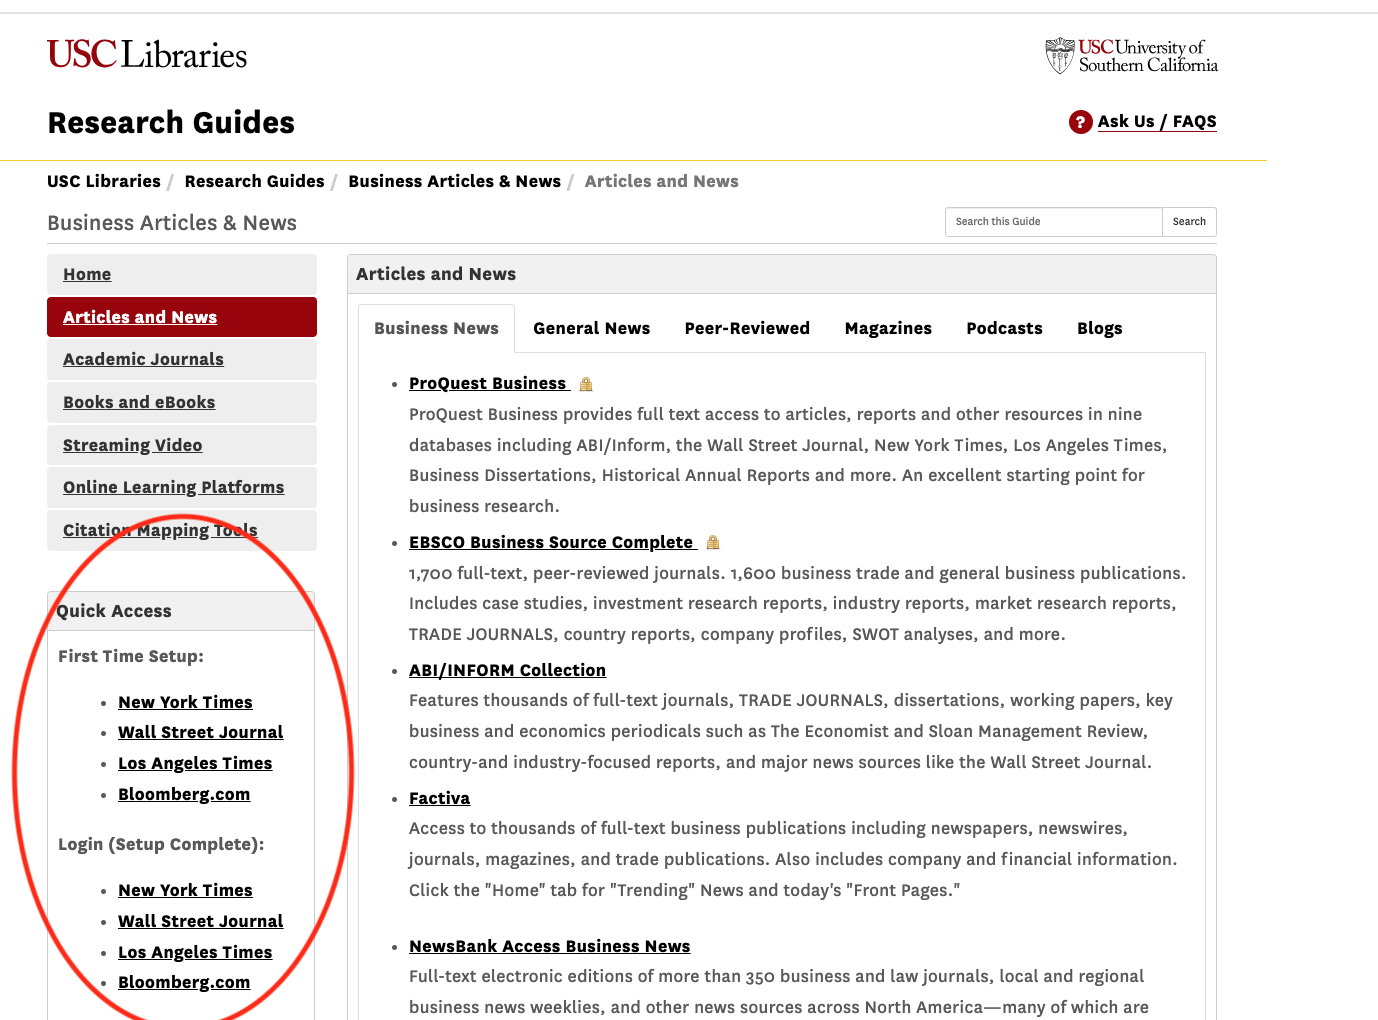
\includegraphics[width=0.7\textwidth]{figures/intro_a_library.png}

\end{frame}

\begin{frame}[t]
    \frametitle{2. Economics 457}
    \framesubtitle{Grading}

    \begin{table}
        \centering
        \caption{Grades for Econ 457}
        \begin{tblr}{
            colspec = {Q[l,wd=2cm] Q[c,wd=2.cm]}
        }
        \toprule
        Item & Percent of Total \\
        \midrule
        Homework & 20\% \\
        Mid-term 1 & 20\% \\
        Mid-term 2 & 25\% \\
        Final & 35\% \\
        \bottomrule
        \end{tblr}
    \end{table}

\end{frame}

\begin{frame}[t]
    \frametitle{2. Economics 457}
    \framesubtitle{Grading}

    Homework
    \begin{itemize}
        \item Goal is to familiarize students with Microsoft Excel, while practicing concepts from class.
        \item 10 assignments.   Best 8 will be counted. (Full points will be given on 2 for free)
        \item 2 points per assigment.   1.5 for turning it on time, 0.5 for getting it (mostly) correct.
        \item Posted and submitted on Brightspace.
        \item Posted on Fridays.  Due at the start of class the following Thursday.   (Brightspace timestamps submissions, late submissions will not be accepted.)
        \item If you'd like to do these in Python/Jupyter, please talk to me after class or in office hours.
    \end{itemize}
\end{frame}

\begin{frame}[t]
    \frametitle{3. Some Interesting Charts}
    \section{Charts}

\end{frame}

\end{document}